\part{Déroulement du stage}
\chapter{Contexte}
\section{Le cloud computing\index{Cloud Computing}}
\subsection{Principe général}
\paragraph*{}
Le \emph{cloud computing} \footnote{Litéralement: "informatique dans les nuages"} est expression
très à la mode ces dernières années et possède une définission très large.
Le principe général est d'externaliser sur des serveurs distants des données ou
des traitements informatiques.

\paragraph*{}
L'avantage pour l'utilisateur du service est qu'il n'a plus à ce soucier d'où se situent physiquement
ses données ni de l'administration des serveurs. Toutes les contraintes de sécurité, de disponibilité
et de fiabilité sont déportées à la responsabilité de l'hébergeur.

\paragraph*{}
Pour l'hébergeur, les avantages sont aussi certain: Le cloud computing permet de mutualiser au maximum
les infrastructures matériels et d'industrialiser une grande partie des processus d'administration.
Par conséquence cette technique permet de diminuer sensiblement les coûts et/ou d'augmenter la qualité
de service.

\subsection{Les différents types de Cloud}

\subsubsection{SaaS\index{SaaS: Software as a Service}}
\paragraph*{}
Le principe du Saas consiste le plus souvent à fournir un service sous la forme d'une application web.
Le type de service rendu est traditionnelement celui que pourrait fournir une application classique.
\\
L'exemple le plus populaire est le webmail\footnote{Interface client de gestion de mail sous forme d'un site web}, comme GMail de Google.

\paragraph*{}
La maintenance des serveurs, de leurs systèmes d'exploitation et des logiciels est faite par le fournisseur de service.
Pour le client, la maintenance ainsi que les MAJ\footnote{MAJ: Mise à jour} des logiciels est transparente et invisible.
\\
Par exemple, personne ne connait le numéro de version de GMail et ça n'interesse personne.

\subsubsection{PaaS\index{PaaS: Platform as a Service}}
\paragraph*{}
Le PaaS est similaire au Saas à la différence que la gestion du logiciel métier est assuré par le client.
Le fournisseur fournit les serveurs et s'occupe de la bonne configuration du système d'exploitation et des middleware
\footnote{Middleware: Logiciel n'étant pas utilisé directement par le client mais par le logiciel métier ou d'autres middlewares} afin
que le logiciel du client fonctionne convenablement.

\paragraph*{}
Alter Way Hosting, est un bon exemple de fournisseur de PaaS: \\
\begin{itemize}
\item 	Le client développe et maintient son site web puis le fournit à AWH.\\
\item 	AWH s'occupe d'acheter, de configurer et de brancher en Data Center\footnote{un Data Center, souvent abbrégé en DC, est une salle
		ou un batiment spécialisé pour y brancher des serveurs} les serveurs puis d'installer et configurer l'OS et les middlewares pour que
		le site web du client fonctionne correctement.
\end{itemize}

\subsubsection{IaaS\index{IaaS: Infrastructure as a Service}}
\paragraph*{}
Dans le cas de l'IaaS, le fournisseur de service, ne s'occupe plus que de founir du matériel au client: serveurs, stockage, réseau...
\\
Ce type d'offre est le plus souvent mise en place gràce à la virtualisation (voir chapitre \ref{virtualisation}) de système d'exploitation.
\\
L'entreprise Amazon, fût pionière dans le domaine de l'IaaS gràce à leur offre d'\textsl{Elastic Compute Cloud}: EC2.

\subsection*{} %To get correct spacement
\begin{figure}
\centering
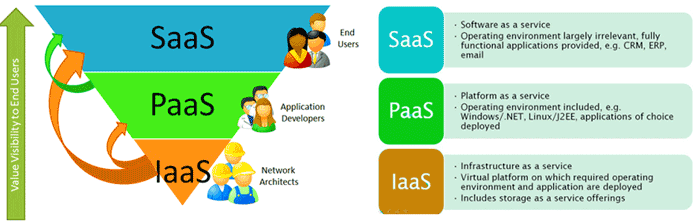
\includegraphics[width=0.9\textwidth]{resource/img/clouds-users}
\caption{Les différents utilisateur du Cloud}
\end{figure}
\begin{figure}
\centering
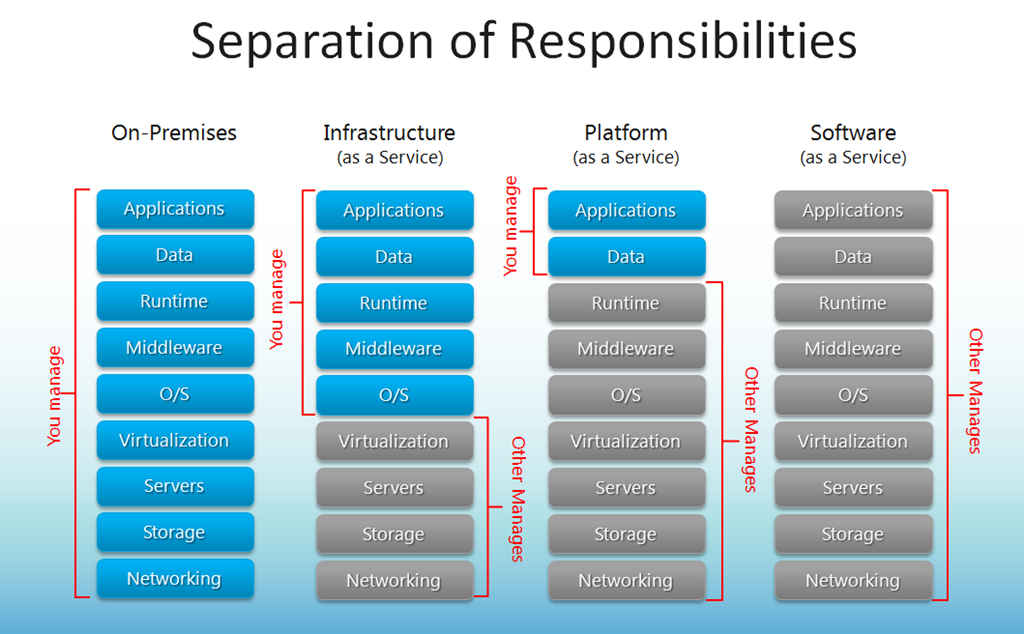
\includegraphics[width=0.9\textwidth]{resource/img/clouds-responsabilities}
\caption{Les différentes responsabilitées des acteurs du Cloud}
\end{figure}

\subsection{Le cloud appliqué à l'hébergement de services ou d'OS\protect\footnote{De l'anglais \textit{Operating System}: Système d'exploitation}}
\paragraph*{}
Le principe du cloud peux être appliqué au niveau du serveur physique et du système d'exploitation. Le responsabilité du fournisseur est de créer/préparer
à la demande du client des machines toutes prêtes avec un système d'exploitation et la bonne configuration réseau.

\paragraph*{}
Souvent, les machines créées ne sont pas des machines physiques mais des machines virtuelles. L'avantage de l'utilisation de machines virtuelles (VM), est
qu'il n'est plus nécéssaire de manipuler physiquement des équipements (serveurs, routeurs, NAS...).
\\
Il est donc possible d'automatiser et d'industrialiser le processus de création d'une nouvelle machine.
\\
Par exemple, sur le site d'amazon, il suffit d'entrer ses coordonnées bancaires et de renseigner quelques options (puissance de la machine, système d'exploitation, logiciels à préinstaller ...)
 pour avoir accès à une machine toute prête en quelques secondes seulement. Ensuite, via un simple clic, il est possible de changer le nombre de machine que l'on veux.
La facturation est calculé à la seconde. Ce type d'offre est donc très pratique pour les personnes ayant besoin de beaucoup de puissance durant un court laps de temps.



\section{La virtualisation}\label{virtualisation}

\section{La problématique d'Alter Way}
\subsection{État actuel des choses}
\paragraph*{}
Le métier d'Alter Way Hosting est principalement de la gestion de serveurs, tant au niveau matériel que logiciel.


\begin{pygmented}{c}
void main(int argc, char* argv[])
{
	printf("hello");
	return 0;
}
\end{pygmented}

\cite{test}
